
\begin{document}

%----------------------------------------------------------------------------------------
%	TITLE PAGE
%----------------------------------------------------------------------------------------

\title[联邦学习]{\huge{联邦学习}  \\
\medskip
\small{Federated Learning}
} % The short title appears at the bottom of every slide, the full title is only on the title page

% \author[文豪]{文豪} % Your name

% \institute[北京航空航天大学] % Your institution as it will appear on the bottom of every slide, may be shorthand to save space
% {
% 数学科学学院 \\ % Your institution for the title page
% \medskip
% \textit{wenh06@gmail.com} % Your email address
% 北京航空航天大学 \\
% 数学科学学院 \qquad 北京航空航天大学
% }

% \logo{\includegraphics[height=1.5cm]{logo}}
% \logoii{\includegraphics[height=1cm]{logo2}}

% \date{\footnotesize 2021年4月13日} % Date, can be changed to a custom date

\setlength{\belowdisplayskip}{5pt} \setlength{\belowdisplayshortskip}{5pt}
\setlength{\abovedisplayskip}{5pt} \setlength{\abovedisplayshortskip}{5pt}

%------------------------------------------------

\begin{frame}
\titlepage % Print the title page as the first slide
\end{frame}

%------------------------------------------------

\begin{frame}
% \frametitle{Overview} % Table of contents slide, comment this block out to remove it
\tableofcontents % Throughout your presentation, if you choose to use \section{} and \subsection{} commands, these will automatically be printed on this slide as an overview of your presentation
\end{frame}

%------------------------------------------------

%------------------------------------------------
%	PRESENTATION SLIDES
%------------------------------------------------


% PPT version (read only share link): https://www.kdocs.cn/l/cigmbsd3uAI4


%------------------------------------------------

\section{引言}

%------------------------------------------------
% Page 1

\begin{frame}
% \frametitle{教育\&工作背景}

联邦学习(Federated Learning)来源于机器(深度)学习模型分布式(Distributed)训练的需求

\begin{figure}
    \centering
    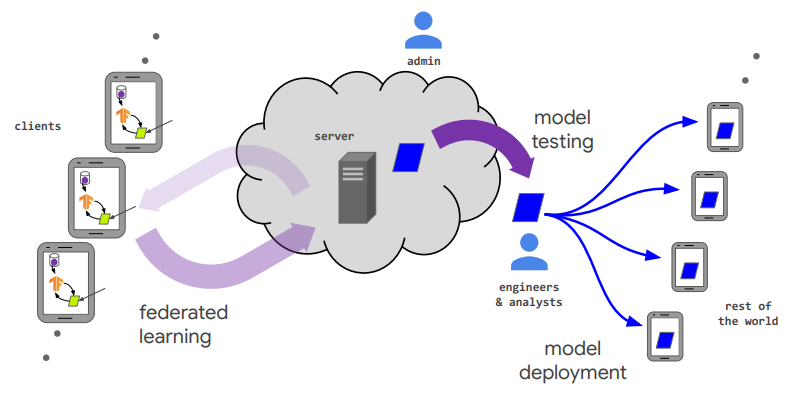
\includegraphics[width=\textwidth,keepaspectratio]{images/fl_overview.png}
\end{figure}

{\footnotesize
图片来源:Kairouz et al., Advances and open problems in federated learning, 2019
}

\end{frame}

%------------------------------------------------
% Page 15

\begin{frame}

Federated Learning这个名词首次由Google的研究人员McMahan等人在文章 \emph{Communication-Efficient Learning of Deep Networks from Decentralized Data} (2017)  中提出。

\vspace{3em}
\pause

相关的分布式的模型训练(优化)方法则可以追溯到更早的时间,例如Boyd等人的 \emph{Distributed Optimization and Statistical Learning via the Alternating Direction Method of Multipliers} (2010)

\end{frame}

%------------------------------------------------
% Page 15

\begin{frame}
\frametitle{参考文献}



\end{frame}


%------------------------------------------------

% \begin{frame}

% \Huge{\centerline{\bfseries The End}}

% \vspace{0.5em}

% \Huge{\centerline{\phantom{a}\bfseries 谢谢!}}

% \end{frame}

%------------------------------------------------

\end{document}
